\documentclass[conference]{IEEEtran}
\usepackage[utf8]{inputenc}
\usepackage[T1]{fontenc}
\usepackage{amsmath,amssymb}
\usepackage{booktabs,tabularx,array}
\usepackage{listings}
\usepackage{xcolor}
\usepackage{tikz}
\usetikzlibrary{arrows.meta,positioning,shapes.geometric,fit,calc}
\usepackage{url}
\usepackage[hidelinks]{hyperref}

\lstdefinestyle{ttl}{basicstyle=\ttfamily\scriptsize,breaklines=true,columns=fullflexible,
  frame=single,framerule=0.2pt,xleftmargin=2pt,xrightmargin=2pt,aboveskip=4pt,belowskip=4pt,
  keywordstyle=\bfseries,morekeywords={INSERT,WHERE,GRAPH,FILTER,NOT,EXISTS,PREFIX,UNION,SELECT}}
\lstset{style=ttl}

\tikzset{
  box/.style={draw,rounded corners=2pt,align=center,font=\scriptsize,inner sep=3pt,minimum height=6mm,fill=gray!8},
  kg/.style={box,fill=blue!10},
  db/.style={box,fill=orange!15},
  app/.style={box,fill=green!10},
  arr/.style={-{Stealth[length=1.6mm]},thick},
  lbl/.style={font=\tiny,midway,fill=white,inner sep=1pt}
}

\begin{document}

\title{A Hybrid Knowledge-Graph and Relational Expert System for Automotive Cost, Contract and Strategy Analysis}

\author{\IEEEauthorblockN{Anjar Tiyo Saputro, Edgar Puyou-Bracq}
\IEEEauthorblockA{Department of Computer Science and Electronics\\
Universitas Gadjah Mada\\
Yogyakarta, Indonesia}}

\maketitle

\begin{abstract}
We present a mini enterprise-resource-planning (ERP) expert system for a car group.
It answers finance, procurement, strategy and sales questions by combining an OWL/RDF knowledge graph, which holds structure and meaning, with a SQLite store, which holds numbers.
The two stores are joined by IRI.
No OWL or SWRL reasoner is used: the original SWRL rules are ported to SPARQL~Update rules that are applied to a fixpoint, which keeps the system small enough to run in a tiny VPS.
The ontology has eight T-Box modules (79 classes, 71 object and 48 datatype properties) and seven A-Box modules, giving 3{,}832 triples after inference.
Nineteen business questions are served by a Rust API, a React interface and a tool-calling language-model chat, and every answer can be traced back to the graph facts that produced it.
All data are synthetic.
\end{abstract}

\begin{IEEEkeywords}
knowledge graph, ontology, T-Box, A-Box, SPARQL, SWRL, rule-based reasoning, expert system, explainable AI
\end{IEEEkeywords}

%--------------------------------------------------------------------
\section{Introduction}
A vehicle group buys thousands of components under supply contracts whose prices follow commodity indices and foreign-exchange (FX) rates.
A decision maker asks questions such as ``rubber is up 15\%: which brand loses most margin?'' or ``which components have a single supplier and no alternative?''
Answering them needs \emph{relationships} (which index drives which contract, which contract covers which component, which model uses it) and \emph{numbers} (index values, prices, volumes).
A relational database alone hides the relationships in join tables; a graph alone is a poor place for time series.

This project builds an expert system that keeps each kind of knowledge in the store that suits it.
Our contributions are:
(i)~a modular ontology for portfolio, sales, contracts, finance, supply terms, risk, market and campaigns;
(ii)~a reasoning layer that replaces an OWL/SWRL reasoner by SPARQL~Update materialisation;
(iii)~a hybrid query design in which the graph finds the explanation path and SQL computes the euro impact;
(iv)~an explainable, deployable application with 19 question services.
\emph{Every supplier, price, contract and result is synthetic and illustrative; nothing describes the real company.}

%--------------------------------------------------------------------
\section{Background}
\textbf{RDF and OWL.} Knowledge is stored as triples $(s,p,o)$. RDFS and OWL add classes, subclass and sub-property axioms, domains and ranges, inverse properties, disjointness and defined classes (\texttt{owl:equivalentClass} with restrictions)~\cite{owl2,rdf}.

\textbf{T-Box and A-Box.} In description-logic terms~\cite{dlhandbook}, the \emph{T-Box} (terminology) contains the schema: classes, properties and axioms such as $\mathit{ElectricModel}\sqsubseteq\mathit{Model}$. The \emph{A-Box} (assertions) contains the individuals and their facts, such as \texttt{vw:ID4 a vw:ElectricModel}. Reasoning derives A-Box facts that follow from the T-Box.

\textbf{SPARQL and SWRL.} SPARQL~1.1~\cite{sparql} queries and, with \texttt{INSERT}~\ldots\texttt{WHERE}, updates a graph. SWRL~\cite{swrl} expresses if-then rules over OWL; it needs a dedicated reasoner.

\textbf{Open versus closed world.} OWL assumes an open world (missing means unknown); an ERP needs a closed-world answer (no contract found means none exists). Materialised SPARQL rules give this closed-world behaviour in a controlled way.

%--------------------------------------------------------------------
\section{Methodology}
We followed an ontology-engineering cycle in the style of Noy and McGuinness~\cite{noy}:
\begin{enumerate}
\item \textbf{Competency questions.} Nineteen target questions fix the scope: finance (5), procurement (4), strategy (5), sales (3) and scenario (2).
\item \textbf{Reuse and extend.} Start from the existing portfolio, sales and contract ontologies; add Finance, Supply, Risk, Market and Campaign modules only where a question needs them.
\item \textbf{Separate by volatility.} \emph{A relationship or classification goes into the graph; a value that changes or is a transaction goes into SQLite.} Prices, planned production and contract terms were first in Turtle and then moved to SQLite (step~8); they are written back to the graph at load time so rules can use them.
\item \textbf{Rules as code.} Inference lives in version-controlled \texttt{.ru} files and is covered by tests.
\item \textbf{Vertical slices.} Eight build steps (spike, rules, skeleton, finance, market, sales, scenario, numeric facts), each delivering data, rules, API, UI and tests.
\end{enumerate}

%--------------------------------------------------------------------
\section{Ontology Design}
The namespace is \texttt{http://example.org/volkswagen/}. Files do not import each other; the application loads each file into its own \emph{named graph}, so provenance (which file asserted a fact) is kept.

\subsection{T-Box}
Table~\ref{tab:tbox} lists the modules. Core design choices:
\begin{itemize}
\item \textbf{Hierarchy.} \texttt{Organization} $\supset$ \texttt{Company}, \texttt{Brand}, \texttt{SeatManufacturer}; \texttt{Offering} $\supset$ \texttt{Product} $\supset$ \texttt{Model}; models are split into \texttt{ElectricModel}, \texttt{HybridModel} and \texttt{CombustionModel}, declared \texttt{owl:AllDisjointClasses}.
\item \textbf{Defined classes.} \texttt{BrandWithElectricModels} $\equiv$ \texttt{Brand} $\sqcap\exists$\texttt{hasModel}.\texttt{ElectricModel}.
\item \textbf{Property axioms.} Inverses (\texttt{hasModel}/\texttt{modelOf}, \texttt{hasIndexationClause}/\texttt{clauseOfContract}); sub-properties (\texttt{hasEngineModel}$\sqsubseteq$\texttt{hasComponent}); typed domains and ranges with \texttt{xsd} datatypes.
\item \textbf{Contract pricing vocabulary.} An \texttt{IndexationClause} links a contract to a \texttt{CommodityIndex} through \texttt{indexedTo}, with \texttt{indexWeight} and \texttt{passThroughRatio} in $[0,1]$.
\item \textbf{Derived vocabulary.} The Risk module declares classes such as \texttt{CommodityExposedContract}, \texttt{FXExposedContract} and \texttt{SingleSourcedCriticalComponent}; \emph{none is asserted}, rules derive them.
\end{itemize}

\begin{table}[t]
\centering\caption{T-Box modules (counts from the Turtle files).}\label{tab:tbox}
\footnotesize
\begin{tabularx}{\columnwidth}{@{}lXrrrr@{}}
\toprule
Module & Scope & Cls & OP & DP & Triples\\
\midrule
VWGroup & group, brand, model, powertrain & 26 & 18 & 8 & 189\\
Sales & clients, leads, matching & 16 & 22 & 15 & 135\\
Contracts & suppliers, components, contracts & 12 & 10 & 11 & 97\\
Finance & currency, profit centre, index & 4 & 3 & 3 & 29\\
Supply & clauses, sourcing, payment & 3 & 6 & 4 & 41\\
Risk & derived exposure classes & 5 & 2 & 0 & 23\\
Market & subsidy, CO$_2$, tariff, rivals & 9 & 7 & 7 & 61\\
Campaign & campaigns, financing & 4 & 3 & 0 & 16\\
\midrule
\multicolumn{2}{@{}l}{Total} & 79 & 71 & 48 & 591\\
\bottomrule
\end{tabularx}
\end{table}

\begin{figure}[t]
\centering
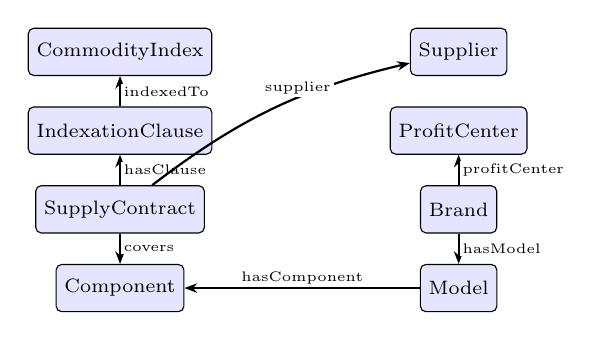
\begin{tikzpicture}[x=1cm,y=1cm]
\node[kg] (idx) at (0,0) {CommodityIndex};
\node[kg] (cl) at (0,-1) {IndexationClause};
\node[kg] (ct) at (0,-2) {SupplyContract};
\node[kg] (co) at (0,-3) {Component};
\node[kg] (md) at (4.3,-3) {Model};
\node[kg] (br) at (4.3,-2) {Brand};
\node[kg] (pc) at (4.3,-1) {ProfitCenter};
\node[kg] (su) at (4.3,0) {Supplier};
\draw[arr] (cl) -- node[lbl,right]{indexedTo} (idx);
\draw[arr] (ct) -- node[lbl,right]{hasClause} (cl);
\draw[arr] (ct) -- node[lbl,right]{covers} (co);
\draw[arr] (md) -- node[lbl,above]{hasComponent} (co);
\draw[arr] (br) -- node[lbl,right]{hasModel} (md);
\draw[arr] (br) -- node[lbl,right]{profitCenter} (pc);
\draw[arr] (ct) to[bend left=12] node[lbl,above,pos=.6]{supplier} (su);
\end{tikzpicture}
\caption{Core T-Box path used by exposure analysis.}\label{fig:tbox}
\end{figure}

\subsection{A-Box}
The A-Box holds 1{,}695 asserted triples (Table~\ref{tab:abox}): the group, brands and models (VWGroup); 24 supply contracts with suppliers, components, currencies and dates; clients and leads; markets and competitors; campaigns; and supply terms. The supply A-Box is \emph{generated} by \texttt{tools/gen\_supply\_abox.py} so that clause tables are edited in one place.
Example (contract 22, tyres, priced in CZK):
\begin{lstlisting}
vw:SupplyContract_22_TyreSet_Standard
  a vw:SupplyContract ;
  vw:contractCoversComponent vw:TyreSet_Standard ;
  vw:contractCurrency vw:CZK ;
  vw:hasIndexationClause vw:Clause_22_NaturalRubber .
vw:Clause_22_NaturalRubber a vw:IndexationClause ;
  vw:indexedTo vw:Index_NaturalRubber ;
  vw:indexWeight "0.40"^^xsd:decimal ;
  vw:passThroughRatio "1.00"^^xsd:decimal .
\end{lstlisting}
\textbf{ERP facts.} Model prices, planned production, contract prices, volumes and discount tiers live in SQLite (13 tables, six numbered migrations) and are written into the graph \texttt{graph/erp-facts} at load (165 triples), so rules see them while SQLite stays the source of truth.

\begin{table}[t]
\centering\caption{Triples by graph role after load.}\label{tab:abox}
\footnotesize
\begin{tabular}{@{}lr@{}}
\toprule
Role & Triples\\
\midrule
T-Box (8 files) & 591\\
A-Box (7 files) & 1{,}695\\
Original SWRL rules (documentation) & 547\\
ERP facts from SQLite & 165\\
Inferred by rules & 834\\
\midrule
Total & 3{,}832\\
\bottomrule
\end{tabular}
\end{table}

%--------------------------------------------------------------------
\section{Reasoning Without a Reasoner}
Neither OWL2-RL nor SWRL is available in the embedded store, and a JVM reasoner would not fit a tiny VPS. We therefore \emph{materialise} inference with SPARQL~Update.

\textbf{Engine.} All files in \texttt{rules/*.ru} are applied in name order, repeatedly, until a full pass adds no triple (a fixpoint). A guard aborts if a maximum number of passes is exceeded. Today the fixpoint is reached in three passes. Each rule file writes to its own graph \texttt{graph/inferred/<file>}, so every inferred edge carries its origin.

\textbf{Rule families.}
\begin{enumerate}
\item \emph{Generic} (\texttt{00}): RDFS/OWL semantics a reasoner would give: sub-property, inverse, subclass and defined-class rules.
\item \emph{Portfolio, contracts, sales} (\texttt{10}--\texttt{30}): the SWRL rules ported to SPARQL (3 portfolio, 2 contract, 10 sales), for example budget, seating and powertrain matching combined into \texttt{suitableModel}.
\item \emph{Exposure and market} (\texttt{40}, \texttt{50}): commodity and FX exposure, single-sourced components, subsidy dependence, CO$_2$ risk.
\end{enumerate}
A representative rule propagates exposure from a contract to a model:
\begin{lstlisting}
INSERT { GRAPH <.../graph/inferred> {
  ?model a vw:CommodityExposedModel ;
         vw:exposedToIndex ?index . } }
WHERE {
  ?model a vw:Model ; vw:hasComponent ?component .
  ?contract vw:contractCoversComponent ?component ;
            vw:exposedToIndex ?index . }
\end{lstlisting}
Chained rules lift exposure from index to clause, contract, component, model, brand and profit centre (Fig.~\ref{fig:tbox}); the fixpoint makes rule file order irrelevant.

\textbf{Trade-offs.} We lose open-world consistency checking and class-satisfiability reasoning, and gain a tiny footprint, predictable run time and rules that are readable and testable. Arithmetic (volume against commitment, discount-tier saving, margin) stays in Rust because SPARQL is a poor calculator for it.

%--------------------------------------------------------------------
\section{System Architecture and Infrastructure}
\begin{figure}[t]
\centering
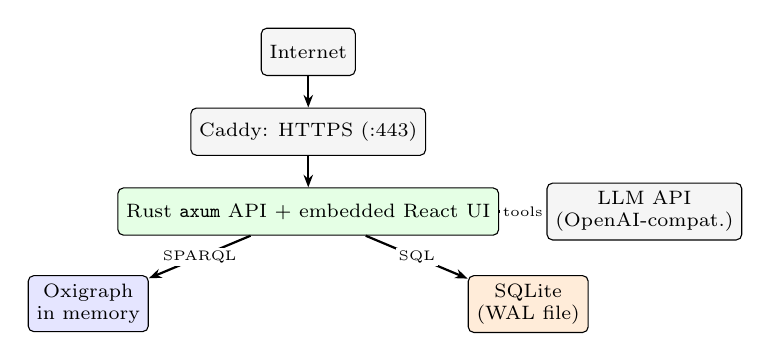
\begin{tikzpicture}[node distance=4mm]
\node[box] (net) {Internet};
\node[box,below=of net] (cad) {Caddy: HTTPS (:443)};
\node[app,below=of cad,minimum width=34mm] (api) {Rust \texttt{axum} API + embedded React UI};
\node[kg,below left=5mm and -4mm of api] (kgs) {Oxigraph\\in memory};
\node[db,below right=5mm and -4mm of api] (sql) {SQLite\\(WAL file)};
\node[box,right=6mm of api] (llm) {LLM API\\(OpenAI-compat.)};
\draw[arr] (net) -- (cad);
\draw[arr] (cad) -- (api);
\draw[arr] (api) -- node[lbl]{SPARQL} (kgs);
\draw[arr] (api) -- node[lbl]{SQL} (sql);
\draw[arr,dashed] (api) -- node[lbl]{tools} (llm);
\end{tikzpicture}
\caption{Production deployment.}\label{fig:arch}
\end{figure}

\textbf{Backend.} A single Rust binary: \texttt{axum} (HTTP/JSON), \texttt{oxigraph} (embedded SPARQL~1.1 store), \texttt{rusqlite}, and \texttt{rust-embed} to serve the compiled UI. Layers: routers (no logic) $\rightarrow$ services (one function per question) $\rightarrow$ adapters (\texttt{kg.rs}, \texttt{db.rs}). Subcommands: \texttt{serve}, \texttt{load-kg}, \texttt{migrate}, \texttt{seed}, \texttt{query}, \texttt{bench}.

\textbf{Why Oxigraph, not GraphDB.} GraphDB is a JVM service needing about 3\,GB RAM for a 2\,GB heap. In our spike, 2{,}263 triples loaded in about 15\,ms with under 9\,MB RSS and mean query latency 0.05--0.5\,ms; the release binary, UI included, is 12.3\,MB. GraphDB is kept only for dev browsing, with an empty or RDFS ruleset so it shows the same triples. The KG is rebuilt from files at every start, so only \texttt{erp.db} needs backup.

\textbf{Frontend.} React, TypeScript, Vite and shadcn/ui; Recharts for charts and Cytoscape.js for the explain graph. Pages: dashboard, scenario lab, contracts, suppliers, markets, sales, models, strategy, explain graph, admin.

\textbf{Deployment.} Multi-stage Docker build (Node builds the UI, Rust builds the binary, a small runtime image runs it). Caddy gives automatic HTTPS and streams server-sent events; the app has its own login. \texttt{make deploy} rsyncs the tree, builds on the server, restarts and checks \texttt{/health}. GitHub Actions runs the web build and \texttt{cargo test} on every pull request and deploys on merge to \texttt{main}.

%--------------------------------------------------------------------
\section{Question Answering and Explainability}
\textbf{Hybrid query flow.} For ``rubber $+15\%$'': (1)~SPARQL walks index $\rightarrow$ clause $\rightarrow$ contract $\rightarrow$ component $\rightarrow$ model $\rightarrow$ brand $\rightarrow$ profit centre; (2)~SQL supplies index series, FX, volume and overhead; (3)~a service merges them. The effective euro price of a contract in month $t$ is
\begin{equation}
P(t)=P_0\Bigl(1+\sum_i w_i\,\rho_i\Bigl(\tfrac{I_i(t)}{I_i(0)}-1\Bigr)\Bigr)\cdot f(t),
\end{equation}
with base price $P_0$, clause weight $w_i$, pass-through $\rho_i$, index $I_i$ and FX factor $f$. For contract~22 the rubber clause ($w=0.40,\rho=1$) means a 15\% rubber rise lifts the tyre price by 6\% before steel and energy.

\textbf{Nineteen questions} (Table~\ref{tab:q}), each a service function, a UI view, a chat tool and a Rust test.

\begin{table}[t]
\centering\caption{Question groups.}\label{tab:q}
\footnotesize
\begin{tabularx}{\columnwidth}{@{}lX@{}}
\toprule
Group & Examples\\
\midrule
Finance (Q1--5) & commodity/FX shock by brand; margin below floor; FX-exposed spend; discount-tier savings\\
Procurement (Q6--9) & supplier failure; single-sourced parts; expiring contracts; lead-time shock\\
Strategy (Q10--14) & subsidy removal; CO$_2$ fleet target; competitor price cut; site dependency; powertrain mix\\
Sales (Q15--17) & hot leads on pressured models; campaigns vs capacity; lease vs loan\\
Scenario (Q18--19) & combined ``bad year''; margin trace\\
\bottomrule
\end{tabularx}
\end{table}

\textbf{Explain graph.} The service \texttt{graph.rs} finds shortest routes between two entities over an allow-list of explanatory predicates, classes each edge as \emph{asserted} (with source file), \emph{inferred} (with rule file) or \emph{ERP fact} (SQLite), and the UI draws them with solid, dashed and dotted lines. Derived shortcuts such as \texttt{exposedToIndex} are excluded so they cannot hide the real chain. Example: rubber $\rightarrow$ clause $\rightarrow$ contract~22 $\rightarrow$ \texttt{TyreSet\_Standard} $\rightarrow$ Golf.

\textbf{Chat with tools.} A chat bubble calls the same services as 21 JSON-schema tools. A language model (any OpenAI-compatible API) chooses tools and writes the answer from their summaries; it never sees SQL or SPARQL, answers only from tool results and states that data are synthetic. The reply is streamed. Without an API key a rule-based planner maps sentences to a tool. The key stays on the server.

%--------------------------------------------------------------------
\section{Evaluation}
\textbf{Correctness.} Rust tests cover rules, every question service, chat tools, the LLM transport (against a local stub) and authentication; the web app is type-checked in CI. The graph service has a test that rejects a spurious route (rubber $\rightarrow$ Euro $\rightarrow$ France $\rightarrow$ Golf).

\textbf{Performance.} Load $\approx$15\,ms (earlier, smaller graph); inference reaches the fixpoint in 3 passes over 3{,}832 triples; memory about 11\,MB while serving.

\textbf{Findings.} (i)~Oxigraph queries see only the default graph, so the adapter sets it to the union of all named graphs. (ii)~\texttt{GROUP\_CONCAT} over IRIs returns nothing; \texttt{STR()} is required. (iii)~Component cost is only 20--40\% of model price, so commodity shocks move margins by tenths of a point. (iv)~Overhead is calibrated so models start at chosen margins; results show the machinery, not facts.

\section{Limitations and Future Work}
Data are synthetic and calibrated. There is no DL consistency checking; revenue delay in Q9 is an upper bound; penalty and renewal clauses are not modelled; rule provenance is per file, not per rule. Future work: a Budget-vs-actual page, HTTP-level tests, a backup scheme (cron or Litestream), a GraphDB triple-count comparison, and measuring LLM answer quality and cost.

\section{Conclusion}
Keeping structure in an ontology and numbers in SQL, and replacing a reasoner by fixpoint SPARQL rules, gives an explainable expert system that runs in a few megabytes. The T-Box/A-Box split, named graphs and rule provenance make each answer traceable from a business number back to graph facts.

\begin{thebibliography}{9}
\bibitem{rdf} W3C, ``RDF 1.1 Concepts and Abstract Syntax,'' 2014.
\bibitem{owl2} W3C, ``OWL 2 Web Ontology Language Document Overview,'' 2nd ed., 2012.
\bibitem{sparql} W3C, ``SPARQL 1.1 Query Language'' and ``SPARQL 1.1 Update,'' 2013.
\bibitem{swrl} I. Horrocks et al., ``SWRL: A Semantic Web Rule Language Combining OWL and RuleML,'' W3C Member Submission, 2004.
\bibitem{dlhandbook} F. Baader et al., Eds., \emph{The Description Logic Handbook}, Cambridge Univ.\ Press, 2007.
\bibitem{noy} N. Noy and D. McGuinness, ``Ontology Development 101: A Guide to Creating Your First Ontology,'' Stanford KSL-01-05, 2001.
\bibitem{oxigraph} T. Pellissier Tanon, ``Oxigraph,'' \url{https://github.com/oxigraph/oxigraph}.
\end{thebibliography}

\end{document}
